% HMC Math dept HW template example
% v0.04 by Eric J. Malm, 10 Mar 2005
\documentclass[12pt,letterpaper,boxed]{hmcpset}

% set 1-inch margins in the document
\usepackage[margin=1in]{geometry}

% include this if you want to import graphics files with /includegraphics
\usepackage{graphicx}

% info for header block in upper right hand corner
\name{Truman Ellis}
\class{CAM 389C}
\assignment{Homework \#1}
% \duedate{09/03/2004}

\begin{document}

% \problemlist{Rudin 3.5, Saff and Snider 1.5.11, 1.7.5ad,\\Dummit and Foote 1.1.25, Logan 1.8.6}

\begin{problem}[Exercise 1.1]
Prove the Kronecker-delta Permutation symbol identities
\begin{align*}
 &\delta_{ii}=3 \,, \\
 &\delta_{ij}\delta_{jk}=\delta_{ik}\,,\\
 &\epsilon_{ijk}\epsilon_{imn}=\delta_{jm}\delta_{kn}-\delta_{jn}\delta_{km}\,,\\
 &\epsilon_{ijk}\epsilon_{ijm}=2\delta_{km}\,,
 &\epsilon_{ijk}\epsilon_{ijk}=6
\end{align*}
\end{problem}

\begin{solution}
\subsection*{$\delta_{ii}=3$}
Using the definition of the Kronecker delta, 
\[
 \delta_{ij}=
\begin{cases} 
1,  & \mbox{if }i=j \\
0,  & \mbox{if }i\neq j
\end{cases}
\]
and summing over the repeated index, $i$,
\[
 \delta_{ii}=\delta_{11}+\delta_{22}+\delta_{33}=3
\]
\subsection*{$\delta_{ij}\delta_{jk}=\delta_{ik}$}
Considering all cases for $i\,,j\,,k$
\begin{align*}
\mbox{case 1}\quad&i=j=k \\
    &1\cdot 1=1\\
\mbox{case 2}\quad&i=j\neq k\\
    &1\cdot 0=0\\
\mbox{case 3}\quad&i\neq j=k\\
    &0\cdot 1=0\\
\mbox{case 4}\quad&i\neq j\neq k\\
    &0\cdot0=0
\end{align*}
All cases have been considered, thus
\[
 \delta_{ij}\delta_{jk}=\delta_{ik}
\]

\end{solution}
% 
% \begin{problem}[SS 1.5.11]
% Solve the equation $(z + 1)^5 = z^5$.
% \end{problem}
% 
% \begin{solution}
% Taking fifth roots of the equation yields
% \[
%   z + 1 = z e^{ik \frac{2\pi}{5}},
% \]
% where $k \in \mathbb{Z}$. We note that $k = 0$ (and all other multiples of 5) yields $z + 1 = z$, which reduces to $1 = 0$, an inconsistent equation. Isolating $z$, we therefore have the solutions
% \[
%   \boxed{z = \frac{1}{e^{ik \frac{2\pi}{5}} - 1},}
% \] 
% with four unique solutions obtained using $k = 1, 2, 3, 4$. We expect 4 unique solutions because $(z + 1)^5 - z^5$ is a fourth-degree polynomial.
% \end{solution}
% 
% \begin{problem}[SS 1.7.5ad]
% Describe the projections on the Riemann sphere of the following sets in the complex plane:
% \begin{itemize}
%   \item[(\textit{a})] the right half-plane $\{ z \mid \text{Re} ~ z > 0 \}$,
%   
%   \item[(\textit{d})] the set $\{ z \mid |z| > 3 \}$.
% \end{itemize}
% \end{problem}
% 
% \begin{solution}[(\textit{a})]
% The right half-plane corresponds to the right open hemisphere $\{ (x_1, x_2, x_3) \in \mathbb{R}^3 \mid x_1 > 0, x_1^2 + x_2^2 + x_3^2 = 1 \}$.
% \end{solution}
% 
% \begin{solution}[(\textit{d})]
% Since $|z| > 3$, $|z|^2 + 1 > 10$, so
% \[
%   x_3 = \frac{|z|^2 - 1}{|z|^2 + 1} 
%   = 1 - \frac{2}{|z|^2 + 1}
%   > 1 - \frac{2}{10} = \frac{4}{5}.
% \]
% Thus, the set $\{ z \mid |z| > 3 \}$ corresponds to the dome of the Riemann sphere above the plane $x_3 = 4/5$. Hand sketches of these projections are shown below:
% 
% \noindent%
% \begin{center}
% \begin{tabular}{cc}
%   (\textit{a}) & (\textit{d}) \\
%   \framebox[1.75in]{\rule{0pt}{1.5in}} & \framebox[1.75in]{\rule{0pt}{1.5in}}  \\
%   \multicolumn{2}{c}{(to be drawn in later)} \\
% \end{tabular}
% \end{center}
% \end{solution}
% 
% \begin{problem}[DF 1.1.25]
% Prove that if $x^2 = 1$ for all $x \in G$ then $G$ is abelian.
% \end{problem}
% 
% \begin{solution}
% Suppose $x^2 = 1$ for all $x \in G$. Then $x = x^2 x^{-1} = 1 x^{-1} = x^{-1}$ for all $x \in G$. For two arbitrary elements $a$ and $b$ of $G$,
% \[
%   ab = (ab)^{-1} = b^{-1} a^{-1} = ba,
% \]
% so $a$ and $b$ commute. Since $a$ and $b$ are arbitrary, $ab = ba$ for all $a$ and $b \in G$, and $G$ is abelian.
% \end{solution}
% 
% %%% sometimes natural pagebreaks separate problem statements from solutions, 
% %%% and we have to change them manually.
% \newpage
% 
% \begin{problem}[Logan 1.8.6]
% This exercise illustrates an important numerical procedure for solving Laplace's equation on a reactangle. Consider Laplace's equation on the rectangle $D: 0 < x < 4, 0 < y < 3$ with boundary conditions given on the bottom and top by $u(x,0) = 0$, $u(x,3) = 0$ for $0 \leq x \leq 4$ and on the sides by $u(0,y) = 2y(3 - y)$, $u(4,y) = 0$ for $0 \leq y \leq 3$. Apply the average value property~(1.45) with $h = 1$ at each of the six lattice points $(1,1), (1,2), (2,1), (2,2), (3,1), (3,2)$ inside $D$ to obtain a system of six equations for the six unknown temperatures on these lattice points. Solve the system to approximate the steady temperature distribution and plot the approximate surface using a software package. 
% \end{problem}
% 
% \begin{solution}
% Applying this average value property with $h = 1$ yields the following linear system:
% \begin{align*}
%   u(1,1) &= \frac{1}{4} (u(1,0) + u(1,2) + u(0,1) + u(2,1)) = \frac{1}{4} (4 + u(1,2) + u(2,1)), \\
%   u(1,2) &= \frac{1}{4} (u(1,1) + u(1,3) + u(0,2) + u(2,2)) = \frac{1}{4} (4 + u(1,1) + u(2,2)), \\
%   u(2,1) &= \frac{1}{4} (u(2,0) + u(2,2) + u(1,1) + u(3,1)) = \frac{1}{4} (u(1,1) + u(2,2) + u(3,1)), \\
%   u(2,2) &= \frac{1}{4} (u(2,1) + u(2,3) + u(1,2) + u(3,2)) = \frac{1}{4} (u(2,1) + u(2,3) + u(3,2)), \\
%   u(3,1) &= \frac{1}{4} (u(3,0) + u(3,2) + u(2,1) + u(4,1)) = \frac{1}{4} (u(3,2) + u(2,1)), \\
%   u(3,2) &= \frac{1}{4} (u(3,1) + u(3,3) + u(2,2) + u(4,2)) = \frac{1}{4} (u(3,1) + u(2,2)),
% \end{align*}
% which we solve in \emph{Mathematica} 5.0 to obtain
% \[
%  \renewcommand{\arraystretch}{1.25}
%   \begin{pmatrix} u(1,1) \\ u(1,2) \\ u(2,1) \\ u(2,2) \\ u(3,1) \\ u(3,2) \end{pmatrix}
%   = \begin{pmatrix} \frac{32}{21} \\ \frac{32}{21} \\ \frac{4}{7} \\ \frac{4}{7} \\ \frac{4}{21} \\ \frac{4}{21} \end{pmatrix}.
% \]
% Plotting these lattice point values yields the following approximate temperature surface:
% \begin{center}
%   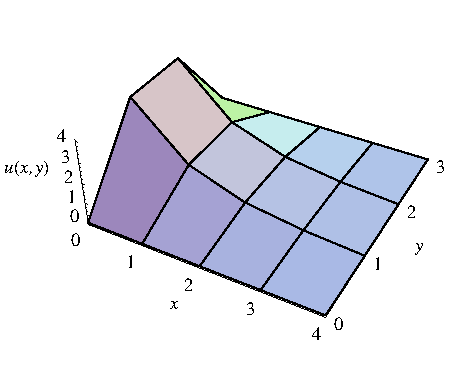
\includegraphics[scale=.8]{logan-1-8-6.pdf}
% \end{center}
% \end{solution}

\end{document}
